\begin{center}
  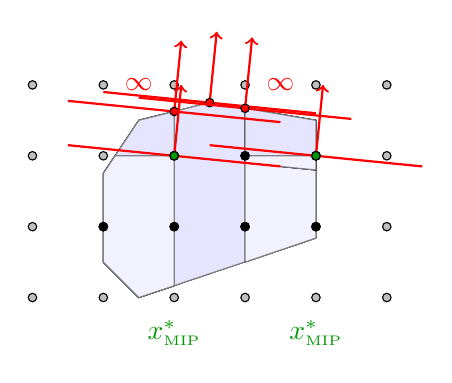
\begin{tikzpicture}[scale=.9]
    \tikzstyle{new} += [draw,fill=blue!20]
    \tikzstyle{old} += [draw=black!50,fill=blue!10]
    \tikzstyle{cutoff} += [draw=black!50,fill=blue!5]

    % --------BOUNDING-BOX--------%
    \draw[white] (0,1) rectangle (5.5,4.8);

    % ----------POLYTOP-----------%
    \visible<1-3>{
      \path[new] (1.0,2.75) -- (1.5,3.5)-- (2.5,3.75) -- (4,3.5) -- (4.0,1.84) -- (1.5,1.0) --(1.0,1.5)--cycle;
    }

    % ----------BranchBound----------%
    \visible<4>{
      \path[old] (1.0,2.75) -- (1.5,3.5)-- (2.5,3.75) -- (4,3.5) -- (4.0,1.84) -- (1.5,1.0) --(1.0,1.5)--cycle;
      \path[new] (3.0,3.67) -- (4,3.5) -- (4.0,1.84) -- (3.0,1.5) -- cycle;
    }
    \visible<4-6>{
      \path[new] (1.0,2.75) -- (1.5,3.5)-- (2.0,3.625) -- (2.0,1.166) -- (1.5,1.0) -- (1.0,1.5) -- cycle;
    }
    \visible<5-11>{
      \path[old] (3.0,3.67) -- (4,3.5) -- (4.0,1.84) -- (3.0,1.5) -- cycle;
    }
    \visible<7>{
      \path[old] (1.0,2.75) -- (1.5,3.5)-- (2.0,3.625) -- (2.0,1.166) -- (1.5,1.0) -- (1.0,1.5) -- cycle;
    }
    \visible<7-10>{
      \path[new] (1.0,2.75) -- (1.166,3.0) -- (2,3) --(2.0,1.166) -- (1.5,1.0) -- (1.0,1.5) -- cycle;
    }
    \visible<11>{
      \path[cutoff] (1.0,2.75) -- (1.166,3.0) -- (2,3) --(2.0,1.166) -- (1.5,1.0) -- (1.0,1.5) -- cycle;
      \path[cutoff] (3.0,2.9) -- (4,2.8) -- (4.0,1.84) -- (3.0,1.5) -- cycle;
    }
    \visible<15-16>{
      \path[new] (3.0,3.67) -- (4,3.5) -- (4.0,2.8) -- (3.0,2.9) -- cycle;
    }
    \visible<12-14,17>{
      \path[old] (3.0,3.67) -- (4,3.5) -- (4.0,2.8) -- (3.0,2.9) -- cycle;
    }
    \visible<17-20>{
      \path[new] (3.0,3) -- (4,3) -- (4.0,2.8) -- (3.0,2.9) -- cycle;
    }
    \visible<21>{
      \path[cutoff] (3.0,3) -- (4,3) -- (4.0,2.8) -- (3.0,2.9) -- cycle;
    }
    
    % ----------GITTER-------------%
    \foreach \x in {0,...,5}
    \foreach \y in {1,...,4}
    {
      \draw[fill=black!25] (\x,\y) circle (0.06);
    }
    % ----------GANZ----------------%
    \foreach \x in {2,3,4}
    \foreach \y in {2,3}
    {
      \draw[fill=black] (\x,\y) circle (0.06);
    }
    \draw[fill=black] (1,2) circle (0.06);


    % ----------OBJECTIVE-----------%
    \visible<3-4>{
      \path[draw=red, thick] (1,3.9) -- (4.0,3.6);
      \path[draw=red,thick,->] (2.5,3.75) -- (2.6,4.75);
      \draw[fill=red] (2.5,3.75) circle (0.06);
    }
    \visible<6-7>{
      \path[draw=red, thick] (0.5,3.775) -- (3.5,3.475);
      \path[draw=red,thick,->] (2.0,3.625) -- (2.1,4.625);
      \draw[fill=red] (2.0,3.625) circle (0.06);
    }
    \visible<9-11>{
      \path[draw=red, thick] (0.5,3.15) -- (3.5,2.85);
      \path[draw=red,thick,->] (2.0,3.0) -- (2.1,4.0);
    }
    \visible<9>{
      \draw [fill=red] (2.0,3.0) circle (0.06);
    }
    \visible<10-19>{
      \draw [fill=green!60!black] (2.0,3.0) circle (0.06);
    }
    \visible<10-19>{
      \node (a) at (2,.5) []{\textcolor{green!60!black}{$x_{\tiny\mbox{MIP}}^{*}$}};
    }
    \visible<12>{
      \node (a) at (1.5,4) []{\textcolor{blue!50}{$\varnothing$}};
    }
    \visible<13-14>{
      \node (a) at (1.5,4) []{\textcolor{red}{$\infty$}};
    }
    \visible<22>{
      \node (a) at (3.5,4) []{\textcolor{blue!50}{$\varnothing$}};
    }
    \visible<23-24>{
      \node (a) at (3.5,4) []{\textcolor{red}{$\infty$}};
    }
    \visible<16-17>{
      \path[draw=red, thick] (1.5,3.82) -- (4.5,3.52);
      \path[draw=red,thick,->] (3,3.67) -- (3.1,4.67);
      \draw [fill=red] (3,3.67) circle (0.06);
    }
    \visible<19-21>{
      \path[draw=red, thick] (2.5,3.15) -- (5.5,2.85);
      \path[draw=red,thick,->] (4,3) -- (4.1,4.0);
      \draw[fill=red] (4,3) circle (0.06);
    }
    \visible<20->{
      \draw[fill=green!60!black] (4,3) circle (0.06);
    }
    \visible<20->{
      \node (a) at (4,.5) []{\textcolor{green!60!black}{$x_{\tiny\mbox{MIP}}^{*}$}};
   }
  \end{tikzpicture}
\end{center}
